% -----------------------------------------------------------------
% Document class: Article
\documentclass[ a4paper, twoside, 11pt]{article}
\usepackage{../../macros-general}
\usepackage{../../macros-article}
% Number of the handout, quiz, exam, etc.
\newcommand{\numero}{01}
\setcounter{numero}{\numero}
\graphicspath{{./figures/}}

% -----------------------------------------------------------------
\begin{document}
\allowdisplaybreaks

% Indices
\newcommand{\iava}{$i$\tsup{ava} }
\newcommand{\iavo}{$i$\tsup{avo} }
\newcommand{\java}{$j$\tsup{ava} }
\newcommand{\javo}{$j$\tsup{avo} }
\newcommand{\kava}{$k$\tsup{ava} }
\newcommand{\kavo}{$k$\tsup{avo} }
\newcommand{\tava}{$t$\tsup{ava} }
\newcommand{\tavo}{$t$\tsup{avo} }
\newcommand{\tmava}{$(t-1)$\tsup{ava} }
\newcommand{\tmavo}{$(t-1)$\tsup{avo} }
\newcommand{\tMava}{$(t+1)$\tsup{ava} }
\newcommand{\tMavo}{$(t+1)$\tsup{avo} }

\begin{center}
\Large Sistemas de Control (EYAG-1005): Tarea \numero \\[1ex]
\small \textbf{Semestre:} 2017-2018 T\'ermino I \qquad
\textbf{Instructores:} Reyes, Leon, Agila, Salazar
\end{center}
\halfskip

\textbf{Ponderaci\'on:} Cada problema equivale a un punto. 
\fullskip

% -----------------------------------------------------------------
\begin{problem}
Un giroscopio es un instrumento para medir velocidades angulares en veh\'iculos aeroespaciales como aviones, cohetes y sat\'elites. Considere el siguiente modelo de un giroscopio de un solo grado de libertad que mide velocidades angulares en el eje-$z$ y produce deflecciones angulares en el eje-$x$, cuya ecuaci\'on diferencial es: \[
J_x \, \ddot{\theta}_x(t) + D_x \, \dot{\theta}_x(t) + K_x \, \theta_x(t)
\,  = \, J \, \omega \, \dot{\theta}_z(t)
\]
\fullcut
\fullcut
\begin{figure}[htb]
\centering
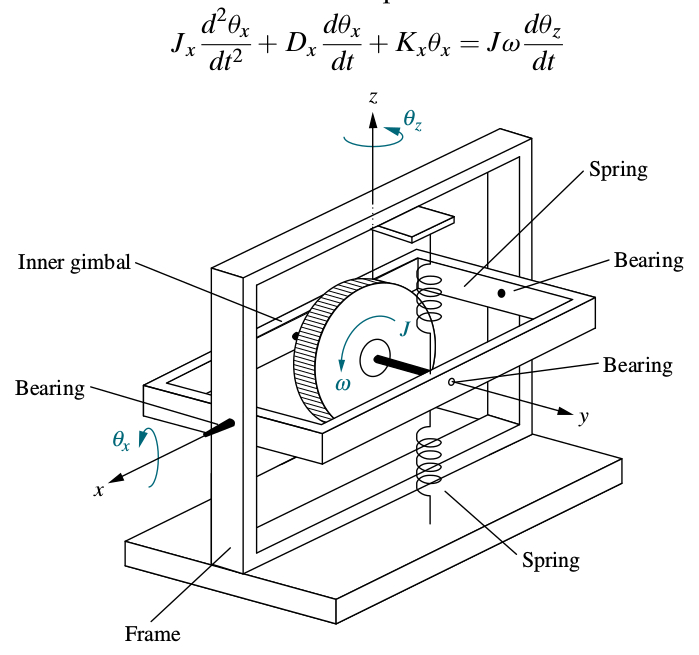
\includegraphics[ width = 0.6\textwidth]{figures/Nise_Prob-3-17.jpg}
\end{figure}

Suponiendo adem\'as que el eje-$x$ est\'a conectado a un potenci\'ometro que indica $C$ voltios por cada grado de deflecci\'on, y denotando al voltage de salida del potenci\'ometro como $v_{pot}(t)$, encuentre la funci\'on de transferencia del giroscopio, \iec
\[
G(s) \, = \, 
\frac{V_{pot}(s)}{\Theta_z(s)}
\]

\end{problem}
\vspace{\baselineskip}

% -----------------------------------------------------------------
\begin{problem}
En el sistema mec\'anico mostrado en la primera figura de la siguiente p\'agina la entrada es el torque $T(t)$ y la salida es el desplazamiento del bloque de masa $x(t)$. \linebreak Encuentre su funci\'on de transferencia, \iec
\[
G(s) \, = \, 
\frac{X(s)}{T(s)}
\]
\begin{figure}[htb]
\centering
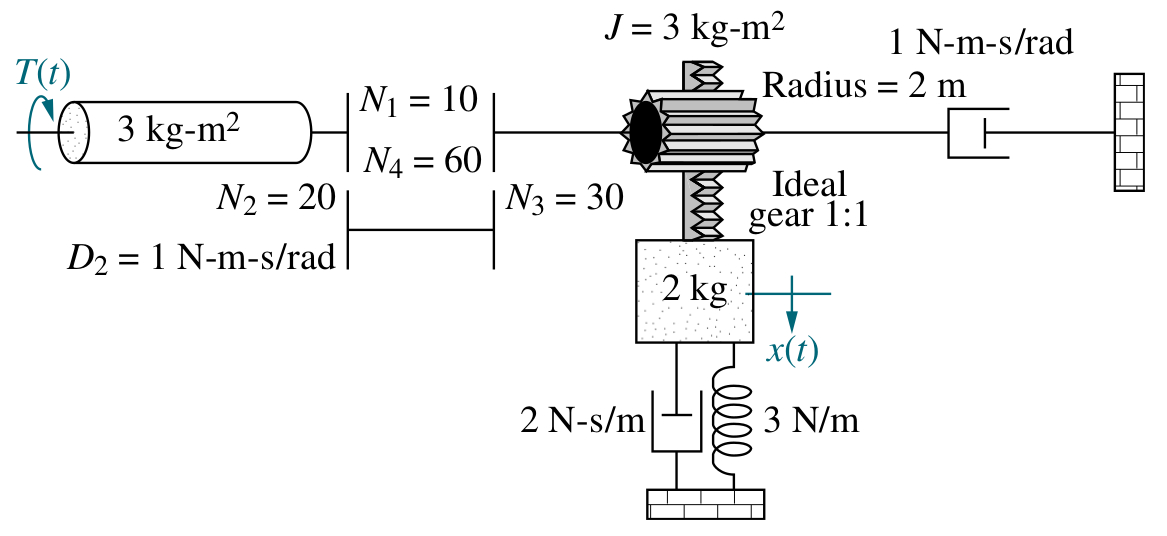
\includegraphics[width=0.68\textwidth]{figures/Nise_Prob-2-40.jpg}
\end{figure}

\end{problem}
\vspace{\baselineskip}

% -----------------------------------------------------------------
\begin{problem}
Considere el sistema mec\'anico rotacional mostrado en la segunda figura de la siguiente p\'agina, donde un motor DC controlado por armadura actua sobre un eje. \linebreak La entrada es el voltage de la armadura $e_a(t)$ y la salida es el desplazamiento angular $\theta_2(t)$. Encuentre su funci\'on de transferencia, \iec
\[
G(s) \, = \, 
\frac{\Theta_2(s)}{E_a(s)}
\]
\emph{Sugerencia:} Para calcular los par\'ametros del motor a partir de la curva torque-RPM refi\'erase a la Secci\'on 2.8 del texto de Nise, ``Electromechanical System Transfer Functions''.

\begin{figure}[ht]
\centering
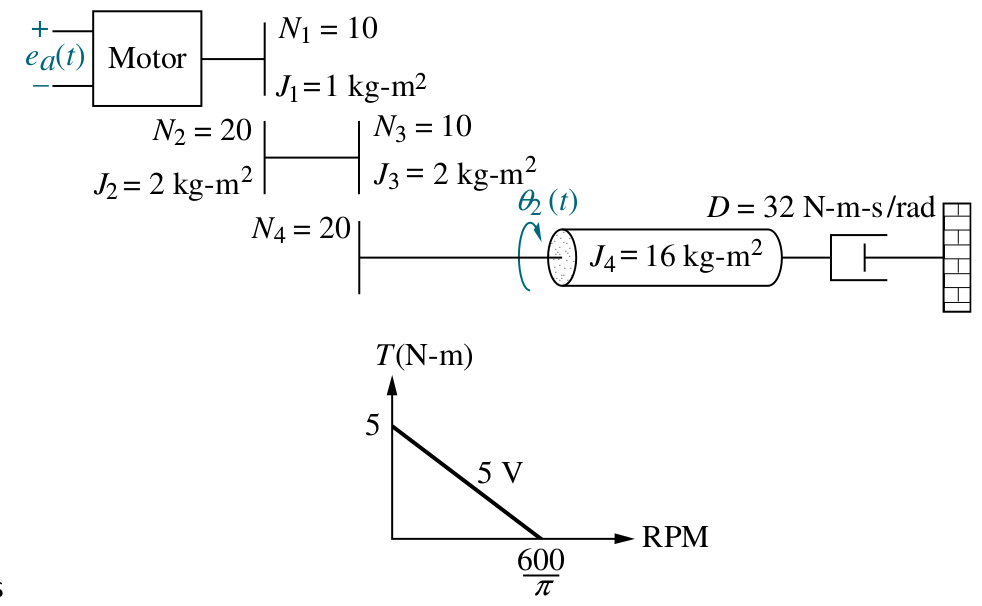
\includegraphics[width=0.66\textwidth]{figures/Nise_Prob-2-43.jpg}
\end{figure}



\end{problem}
\vspace{\baselineskip}

% -----------------------------------------------------------------
\begin{problem}
Dado el siguiente sistema encuentre su funci\'on de transferencia en circuito cerrado como funci\'on de las funciones de transferencia de sus subsistemas. 

\begin{figure}[htb]
\centering
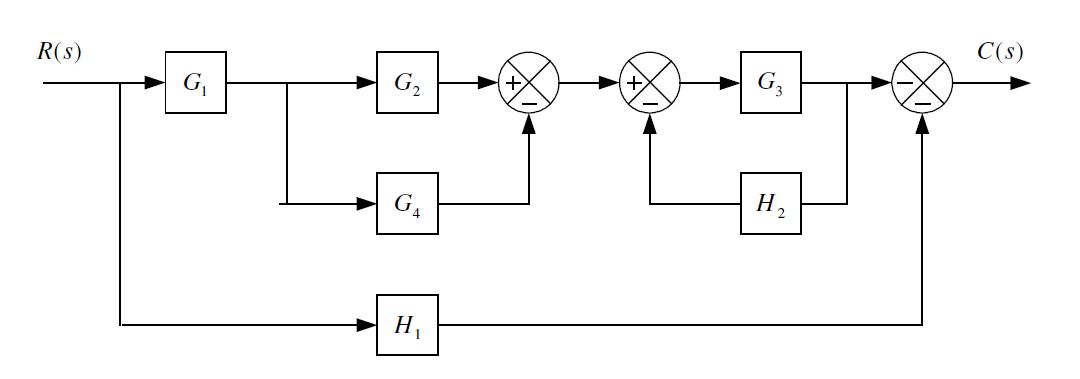
\includegraphics[width=0.88\textwidth]{figures/bloques2.JPG}
\end{figure}

\end{problem}
\vspace{\baselineskip}

% -----------------------------------------------------------------
\begin{problem}
Para el sistema en la primera figura de la siguiente p\'agina encuentre la funci\'on de transferencia en circuito cerrado como funci\'on de las funciones de transferencia de sus subsistemas. 

\begin{figure}[htb]
\centering
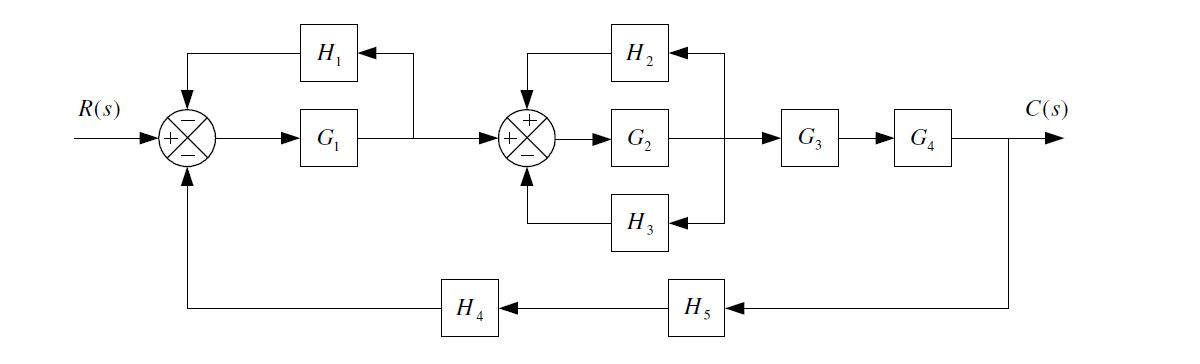
\includegraphics[width=\textwidth]{figures/bloques3.JPG}
\end{figure}

\end{problem}
\vspace{\baselineskip}

% -----------------------------------------------------------------
\begin{problem}
Para el sistema de control de direcci\'on de un veh\'iculo terrestre mostrado en la segunda figura de la siguiente p\'agina, encuentre su funci\'on de transferencia en circuito cerrado como funci\'on de $K$. 

\begin{figure}[H]
\centering
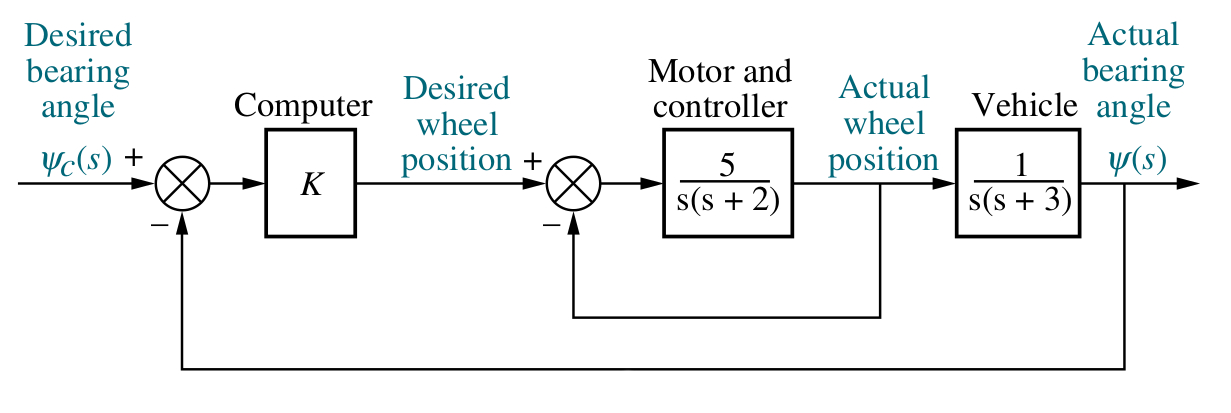
\includegraphics[width=0.74\textwidth]{figures/Nise_Prob-5-51.jpg}
\end{figure}

\end{problem}
\vspace{\baselineskip}

% -----------------------------------------------------------------
\begin{problem}
Considere el sistema de control de posici\'on angular mostrado en la figura de abajo. Encuentre valores para las ganancias $K_1$ y $K_f$ de tal manera que las m\'etricas de respuesta en el tiempo del sistema en circuito cerrado sean: 
\begin{itemize}
\item Porcentaje de sobrepaso del 25\%. 
\item Tiempo de asentamiento de 0.2 segundos. 
\end{itemize}
Adem\'as, calcule el error en estado estable del sistema para:
\begin{itemize}
\item Una entrada escal\'on $r(t) \, = \, C_1 \, u(t)$.
\item Una entrada rampa $r(t) \, = \, C_2 \, t \, u(t)$. 
\end{itemize}
\begin{figure}[H]
\centering
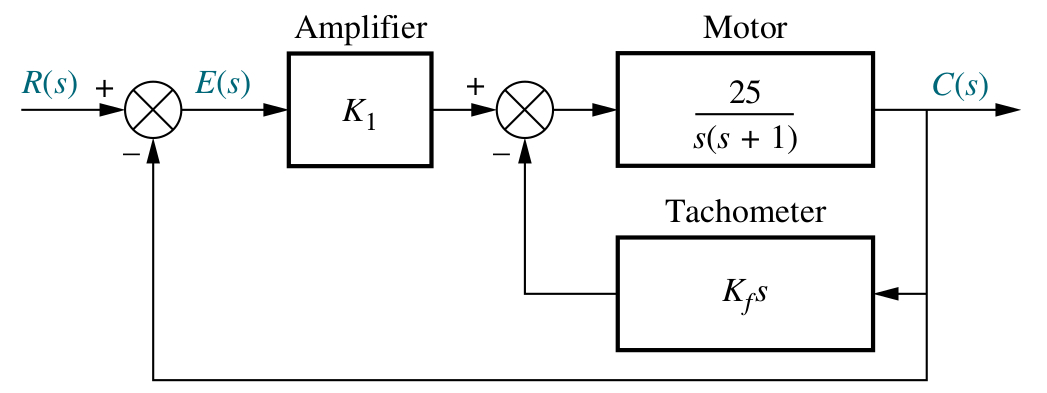
\includegraphics[ width = 0.6\textwidth]{figures/fig_P9-8.jpg}
\end{figure}

\end{problem}
\vspace{\baselineskip}

% -----------------------------------------------------------------
\begin{problem}
Considere el sistema de control de cabeceo de un veh\'iculo a\'ereo no-tripulado mostrado en la primera figura de la siguiente p\'agina. 
\begin{enumerate}[label=\alph*.]
\item Asumiendo la forma del controlador mostrada en la figura, bosqueje el lugar geom\'etrico de las ra\'ices \emph{(root locus)}. 
\item De acuerdo a su bosquejo anterior, determine la veracidad o falsedad de cada uno de las siguientes proposiciones. 
\begin{itemize}
\item El sistema es estable para todo valor de la ganancia $K$. 
\item Existe un valor de $K$ tal que si $K$ excede ese valor entonces el sistema es inestable. 
\item Existe un valor de $K$ para el cual todos los polos del sistema son complejos. 
\item Existe un valor de $K$ para el cual todos los polos del sistema son reales. 
\end{itemize}

\begin{figure}[htb]
\centering
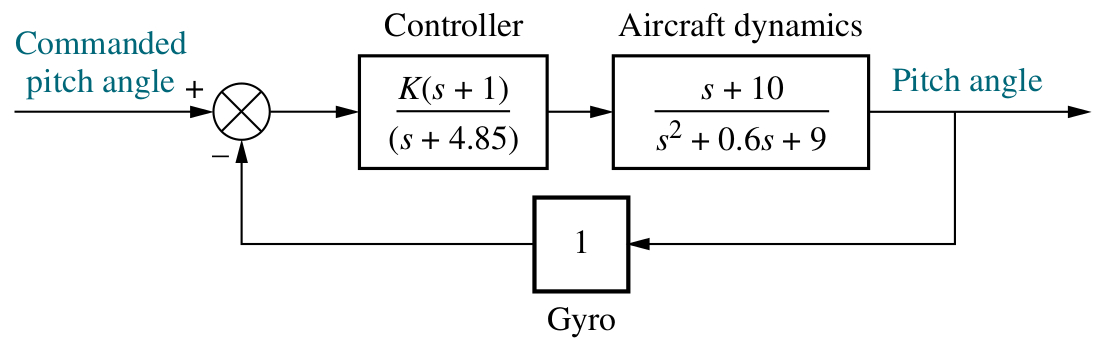
\includegraphics[ width = 0.64\textwidth]{figures/fig_P6-12.jpg}
\end{figure}

\end{enumerate}

\end{problem}
\vspace{\baselineskip}

% -----------------------------------------------------------------
\begin{problem}
Para siguiente sistema de control angular encuentre valores para las ganancias $K_1$ y $K_2$ tales que en circuito cerrado el sistema tenga las siguientes caracter\'isticas: 
\begin{itemize}
\item Tasa de amortiguamiento $\zeta = 0.5$. 
\item Error en estado estable $e(\infty) = 0.1 \, C$ para una entrada rampa $r(t) \, = \, C \, t \, u(t)$. 
\end{itemize}

\begin{figure}[htb]
\centering
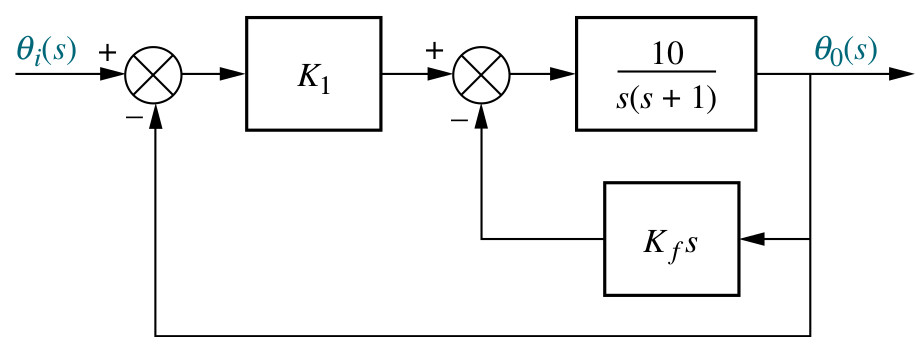
\includegraphics[ width = 0.52\textwidth]{figures/fig_P7-35.jpg}
\end{figure}

\end{problem}
\vspace{\baselineskip}

% -----------------------------------------------------------------
\begin{problem}
Estime la funci\'on de transferencia del sistema de segundo orden cuya respuesta a una entrada escal\'on es como se muestra abajo: 
\fullskip

\begin{figure}[htb]
\centering
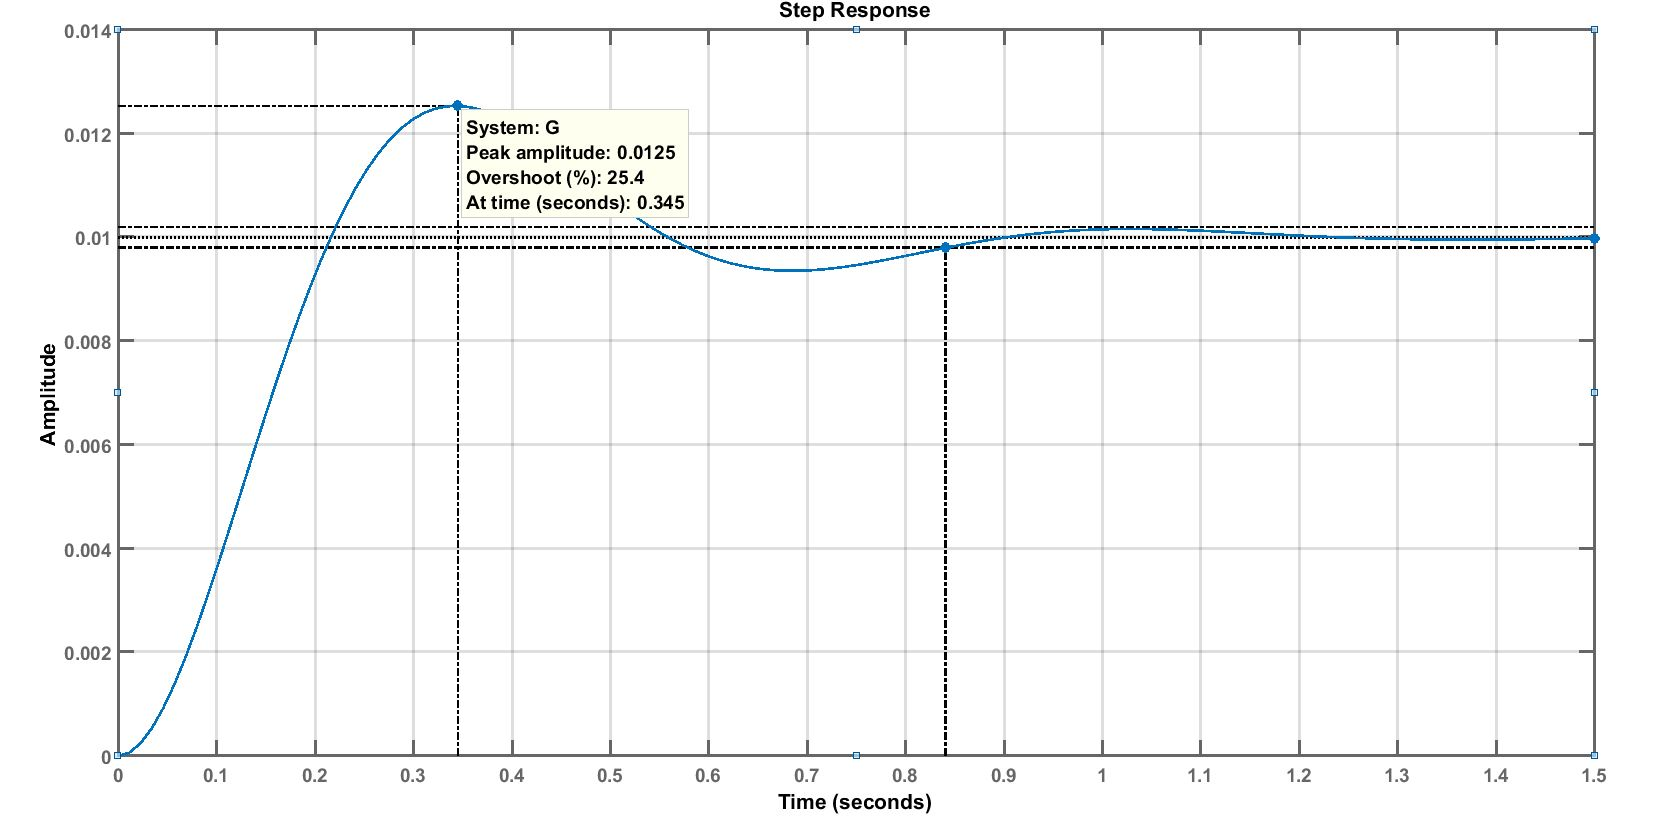
\includegraphics[ width = \textwidth]{figures/especificaciones.JPG}
\end{figure}

\end{problem}
\vspace{\baselineskip}

\end{document}
